\section{Übungsaufgaben: Asymmetrische Kryptologie}
\subsection{Rucksack}


PrivateKey: $(3,5,10,23), m= 8	, n = 47$

\subsubsection{Geben sie den öffentlichen Schlüssel an}

\begin{align}
	 3 \cdot 8 \mod 47 &= 24 \\
  	 5 \cdot 8 \mod 47 &= 40 \\
	10 \cdot 8 \mod 47 &= 33 \\
	23 \cdot 8 \mod 47 &= 43 	
\end{align}

PublicKey: $(24,40,33,43)$

\subsubsection{Verschlüsseln Sie $P=[1110 0000 0010]_2$ (Binärdarstellung) im ECB-Modus.}


\begin{align}
	C_1 = 1 \cdot 24 + 1  \cdot  40 + 1 \cdot 33 +0  \cdot 43 &= 97 \\ 
	C_2 = 0 \cdot 24 + 0  \cdot  40 + 0 \cdot 33 +0  \cdot 43 &= 0   \\ 	
	C_3 = 0 \cdot 24 + 0  \cdot  40 + 0 \cdot 33 +0  \cdot 43 &= 33 
\end{align}


\subsubsection{Finden Sie den Plaintext zum Ciphertext $C = (67, 64)$}


$m^{-1} = 6$:

$C_1= 67 * 6 \mod 47 = 26$

\begin{tabular}{ccc}
 $S_i$ & $Cm^{-1}$ & $P$ \\ \hline
 23    & 26  & 1  \\
 10    & 3   & 0  \\
 5     & 3   & 0  \\
 3     & 0   & 1  
\end{tabular}

\textbf{Kein gültiger Ciphertext}

$C_2= 64 * 6 \mod 47 = 8$

\begin{tabular}{ccc}
 $S_i$ & $Cm^{-1}$ & $P$ \\ \hline
 23    & 8  & 0  \\
 10    & 8  & 0  \\
 5     & 3  & 1  \\
 3     & 0   & 1  
\end{tabular}

$P_2 = 0011$

\subsection{RSA auf Nachricht in Blöcken}
\begin{align}
  P &= \text{'FHT4EVER'}  &
  n &= 13 \cdot 17 = 221 & e &= 3
\end{align}

\textbf{Beachten: $ggT(e, \phi(221) ) \ne 1$}. Entschlüsselung damit ummöligch.

\begin{align}
	E(x) &=  x^3 \mod 221 \\
	E(P) &=  E('F') \circ E('H')\circ E('T')\circ E('4')\circ E('E')\circ E('V')\circ E('E')\circ E('R')\\
		 &=  \operatorname{apply}(x^3 \mod 221 ,[70, 72, 84, 52, 69, 86, 69, 82])    \\
		 &=  [8, 200, 203, 52, 103, 18, 103, 194]
\end{align}


\subsection{Chinesischer Restsatz}
\subsubsection{Es sei $m = 11, n = 12, a = 3$ und $b = 4$. Geben Sie ein $x$ an, für das gilt: $x \mod m = a$ und $ x \mod n = b$}

\begin{equation}
	x = a n N + b m M  = 3 \cdot 12 \cdot N + 4 \cdot 11 M
\end{equation}

$$ggT(12, 11) = 1 \text{ mit } a^{-1} = -1 = N$$
$$ggT(11, 12) = 1 \text{ mit } a^{-1} =  1 = M$$

\begin{align}
	X &= 3 \cdot 12 \cdot 1 + 4 \cdot 11 \cdot -1 \\
	  &=  36 - 44 = -8
\end{align}
\textbf{Probe:}
\begin{align}
	-8 \mod  m &= a  & -8 \mod  n &= b \\
	-8 \mod 11 &= 3  & -8 \mod 12 &= 4 \\
\end{align}

\subsubsection{Es sei $m = 11, n = 12, l = 12, a = 3, b = 4 \text{ und } c=5$. Geben Sie ein $x$ an, für das
gilt: $x \mod m = a$ und $x \mod n = b$ und $x \mod l = c$.}

\begin{align}
 X = a \cdot n \cdot l (nl)^{-1}
   + b \cdot m \cdot l (ml)^{-1}
   + c \cdot n \cdot m (nm)^{-1} \\
 x \mod 11 = 3 \\
  x \mod 12 &= 4\\
   x \mod 11 &= 5\\
\end{align}




\textbf{Vorrausetzung für Chin. Restsatz nicht erfüllt.}
$ggT(n,l)=12$ damit nicht relativ prim.


\subsubsection{Verallgemeinern Sie den Chinesischer Restsatz:
Gesucht ist $x$ mit $(x \mod m_i)=x_i$ und die passende Berechnungsvorschrift. Wie groß ist die Laufzeit zur Berechnung von x?}

\textbf{Eingabe}: $m_i$ die Module (paarweise relativ prim), $x_i$ die gesuchten Ergebnisse mit $1 \le i \le n$. 

Sei $N_j$ das Produkt von $ \prod_{i>0 \wedge i \ne j}^{n} m_i = 
	m_1 \cdots m_{j-1} \cdot m_{j+1} \cdots m_n$	
Sei $M_i$ multiplikative Inverse von $N_i$ zu $m_i$.

\begin{align}
	X &= \sum_{i}^{n} x_i \underbrace{N_i M_i}_{\equiv_{m_i} 1} \\
	  &= x_1 m_2 \cdots m_n M_1 + \ldots + x_n m_1 \cdots m_{n-1} M_n	
\end{align}

Kosten: $T = n \cdot T_{\text{egcd}} + n (n+1) T_{\text{mult}} + n T_{\text{add}} \in \mathcal{O}(n^2)$.

\subsection{RSA-Low-Exponent-Attack}
\subsubsection{Gg. seien die drei öffentlichen RSA-Schlüssel $(n_1 = 35,e=3)$,$(n_1 = 35,e=3)$,$(n_1 = 35,e=3)$.
Außerdem bekannt ist: $C_{123}=(22,12,216)$}

Voraussetzungen: 
	$$ C_{123} = P^3 \mod n_{123} $$
und $n_{123}$ sind paarweise relativ prim.

Gesucht $x$:
$$ x \mod n_{1} = C_{1} \wedge
   x \mod n_{2} = C_{2} \wedge
   x \mod n_{3} = C_{3} \wedge   $$

\begin{align}
	x = \underbrace{C_{1} n_{2} n_{3} N_{23}}_{\equiv 1 \mod n_1}
	  + \underbrace{C_{1} n_{1} n_{3} N_{13}}_{\equiv 1 \mod n_2}
	  + \underbrace{C_{1} n_{1} n_{2} N_{12}}_{\equiv 1 \mod n_3}
\end{align}

Suche der multiplikativen Inversen $N_{123}$ zum Modul $n_{123}$ mit erweiterter euklidischer Algorithmus:

$ggT(n_{2}n_{3},n_{1}) = ggT(24,35):$
\begin{align}
35 &= 1 \cdot 24+11			\\
24 &= 2 \cdot 11+2			\\
11 &= 5 \cdot 2+1			
\end{align}

\begin{align}
1 &= 11 - 5 \cdot 2						\\
1 &= 35 -24 - 5 \cdot (24-2 \cdot 11)	\\
1 &= -24 -5 \cdot (24-2 \cdot (35-24))  \\
1 &= -24 -5 \cdot (24+2 \cdot 24)		\\
1 &= -16 \cdot 24						\\
1 &=  19 \cdot 24						
\end{align}

$$N_{23} = 19$$

$ggT(n_{1}n_{3}, n_{2}) = ggT(8,143):$
\begin{align}
134   &= 17 \cdot 8+7			\\
8     &= 7+1
\end{align}

\begin{align}
1 = 8 -7						\\
1 = 8 -(143-17 \cdot 8)			\\
1 = 8+17 \cdot 8				\\
1 = 18 \cdot 8					
\end{align}

$$N_{13} = 18$$

$ggT(n_{1}n_{2}, n_{3}) = ggT(160,323):$
\begin{align}
323 = 2 \cdot 160+3\\
160 = 53 \cdot 3+1\\
\end{align}
\begin{align}
1 = 160-53 \cdot 3 \\
1 = 160-53 \cdot (323-2 \cdot 160) \\
1 = 107 \cdot 160
\end{align}

$$N_{12}= 107$$
	
\begin{equation}
	x = P^3 = 137.424.442 = 12.167 (mod n_{1}n_{2}n_{3})
\end{equation}
\begin{equation}
P=  \sqrt[3]{x} = \sqrt[3]{12167} = 23
\end{equation}

\textbf{Probe:}
\begin{equation}
23^3 \mod n_{123} = C_{123}
\end{equation}



\subsubsection{}

\subsection{Quadratwurzeln mod n}
				\[ 16 \mod 35 \]				
\subsubsection{mit chin. Restsatz}

Zerlegung in $pq=n$ mit $7 \cdot 5 = 35$.

Lösung von $16  \equiv 2 \mod 7$ mit Folgerung (2.5).

\[ 2^{\dfrac{7+1}{4}}  \imp x_1 = 4 \wedge x_2 = 7 - 4 = 3 \]

Lösung von $16 \equiv 1 \mod 5$:

\[ x_3 = 1 \text{ und } x_4 = 4 \]

\begin{align}
	x & = 1 \mod 5 \label{eq:bbb}\\
	x & = 3 \mod 7 \label{eq:bba}\\ 
	x & = 4 \mod 7 \label{eq:bbc}\\
	x & = 4 \mod 5 
\end{align}

Betrachtung für  \eqref{eq:bbb} mit  \eqref{eq:bba} und \eqref{eq:bbc}  reicht:

\begin{equation}
	X = x_1 p P + x_2 q Q = 1 \cdot 7 P + 3 \cdot 5 Q
\end{equation}

$ggT(7,5)=1 a^{-1} = 3$
$ggT(5,7)=1 a^{-1} = 10$

\[	X_1 = 4\]


\begin{equation}
	X = x_3 p P + x_3 q Q = 4 \cdot 7 P + 4 \cdot 5 Q
\end{equation}

$ggT(7,5)=1 a^{-1} = 3$
$ggT(5,7)=1 a^{-1} = 10$

\[	X_2 = 9\]

Weitere \[X_3 = 35-X_1 = 31 \text{ und } X_4 = 35-X_2 \]
 
\subsubsection{}
[0, 1, 4, 9, 16, 25, 1, 14, 29, 11, 30, 16, 4, 29, 21, 15, 11, 9, 9, 11, 15, 21, 29, 4, 16, 30, 11, 29, 14, 1, 25, 16, 9, 4, 1]

\subsection{Rabin}

Sei der öffentliche Schlüssel $n=77$, der geheime Schlüssel $p=7$ und $q=11$.
Gegeben sei der Ciphertext $C = 23$.
\subsubsection{Wie lauten die möglichen Klartexte?)

Lösung für $x^2 \equiv_p C$ (2.5):    

\begin{equation}
	C^{\dfrac{7+1}{4}} \equiv_7 = 4
\end{equation}

\[ x_{12} = 4,3 \]

Lösung für $x^2 \equiv_q C$ (2.5):    

\begin{equation}
	C^{\dfrac{11+1}{4}} \equiv_11 = 1
\end{equation}

\[ x_{34} = 1,10 \]

Mit dem Restsatz: \[X = (32,45,10,67)\]

\subsubsection{Sie wissen, dass der Klartext in seiner 7-Bit-Binärdaretsllung im höchsten Bit
eine „1“ hat. Welches ist der gesuchte Klartext?}

$P=67$

\subsection{Elgamal}
Öffentlicher Schlüssel: $p = 2579$, Primitivwurzel $g = 2, y = 2765 = 949 \mod 2579$ \\
Geheimer Schlüssel: $x = 765$ \\
Nachricht: $m = 1299, k = 853$\\
\subsubsection{Führen Sie die Verschlüsselung durch.}

\begin{align}
	a&= g^k \mod p = 2^{853} \mod 2579 = 453 \\
	b&= y^km \mod p = 949^{853} \cdot 1299 \mod 2579 =2396
\end{align}

\[ C= (453,2396) \]

\subsubsection{Führen Sie die Entschlüsselung des Ciphertexts durch und überprüfen Sie, ob
Sie wieder m erhalten.}

\begin{align}
	P = \dfrac{b}{a^x} \mod 2579= \dfrac{2396}{453^{765}} \mod 2579 = 5 
\end{align}
\textbf{WTF!}

\subsection{Diskrete Exponential-Funktion}


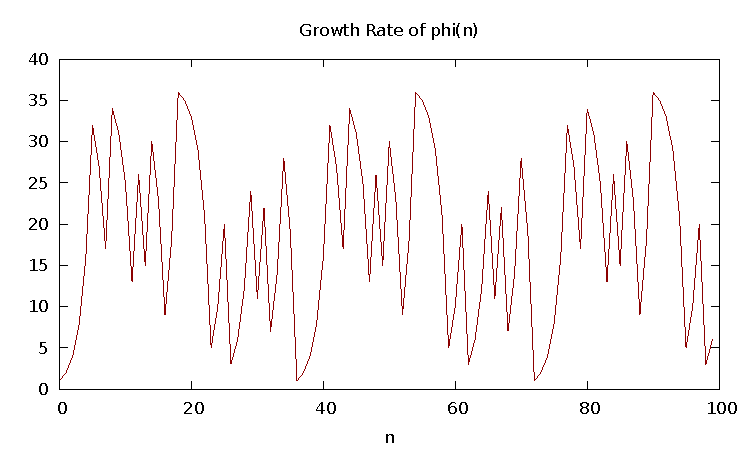
\includegraphics[scale=1]{eclipse/expofun.pdf}

\subsection{Primfaktorzerlegung}
\subsection{Fermatscher Primzahltest}
\subsection{Inverses zu ($n-1) \mod n$}
\subsection{$a(n-1) \mod n$}
\subsection{$\phi(n)$ für $n < 500$}

\subsubsection{Berechnen Sie $\phi(n)$ für $n < 500$ und tragen Sie die Werte in einem Graphen}

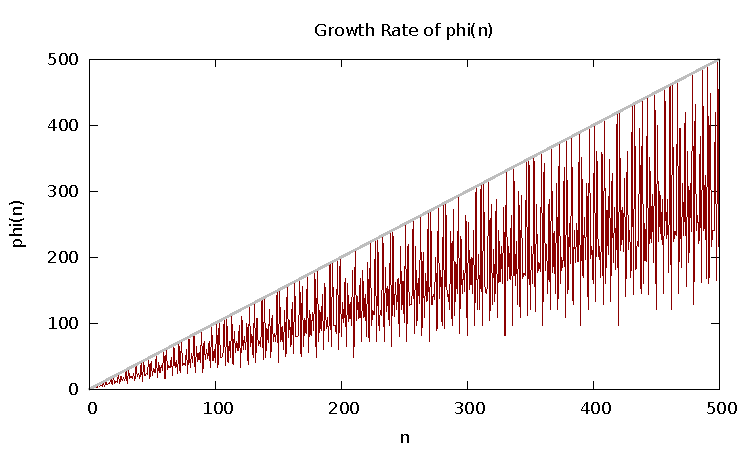
\includegraphics[scale=1]{eclipse/growth-rate.pdf}

\subsubsection{Geben Sie eine möglichst genaue obere Schranke für $\phi(n)$ an.}

\begin{align}
	 \phi(n) &\le n-1 \\
	 & \in \mathcal{O}(n)
\end{align}	
